\documentclass[tikz,border=6pt]{standalone}
\usepackage[T1]{fontenc}
\usepackage{lmodern}
\usepackage{amsmath}
\usepackage{amssymb}
\usepackage{bm}
\usepackage{xcolor}
\usepackage{tikz}
\usetikzlibrary{arrows.meta,positioning,fit,calc,backgrounds,shapes.multipart,shapes.geometric}

\colorlet{mandalaBlue}{blue!55!black}
\colorlet{mandalaTeal}{teal!55!black}
\colorlet{mandalaGreen}{green!45!black}
\colorlet{mandalaGold}{orange!70!black}
\colorlet{mandalaRed}{red!55!black}
\colorlet{mandalaViolet}{violet!55!black}
\colorlet{mandalaGray}{black!55}
\colorlet{mandalaLight}{black!3}

\tikzset{
  >=Latex,
  font=\sffamily,
  % Color semantics used consistently across all diagrams:
  % mandalaBlue   -> external inputs / sources / configuration
  % mandalaTeal   -> internal data containers / encoded features
  % mandalaGreen  -> geometric or physics-aware transformations
  % mandalaGold   -> model computation or linear-algebra solve stages
  % mandalaViolet -> predicted operator-valued objects and heads
  % mandalaRed    -> optimization / objectives / losses
  titlebox/.style={
    rounded corners=2.5pt,
    fill=mandalaBlue!8,
    draw=mandalaBlue,
    line width=0.8pt,
    inner sep=6pt,
    minimum height=10mm,
    align=center,
    font=\sffamily\bfseries\large
  },
  panel/.style={
    rounded corners=3pt,
    fill=white,
    draw=black!45,
    line width=0.8pt,
    inner sep=5pt
  },
  stage/.style={
    rounded corners=3pt,
    fill=#1!10,
    draw=#1!85!black,
    line width=0.9pt,
    minimum width=32mm,
    minimum height=11mm,
    align=center,
    font=\sffamily\small
  },
  stage/.default=mandalaBlue,
  smallstage/.style={
    rounded corners=2.5pt,
    fill=#1!9,
    draw=#1!80!black,
    line width=0.75pt,
    minimum width=27mm,
    minimum height=8.5mm,
    align=center,
    font=\sffamily\scriptsize
  },
  smallstage/.default=mandalaBlue,
  sidepanel/.style={
    rounded corners=3pt,
    fill=#1!8,
    draw=#1!75!black,
    line width=0.8pt,
    inner sep=5pt,
    align=left,
    font=\sffamily\scriptsize,
    text width=43mm
  },
  sidepanel/.default=mandalaTeal,
  annot/.style={
    font=\sffamily\scriptsize,
    text=mandalaGray,
    align=left
  },
  arrow/.style={
    -{Latex[length=2.6mm,width=1.8mm]},
    line width=0.95pt,
    draw=black!70
  },
  dashedarrow/.style={
    -{Latex[length=2.4mm,width=1.7mm]},
    line width=0.85pt,
    draw=black!65,
    dashed
  },
  softfit/.style={
    rounded corners=4pt,
    draw=black!35,
    fill=black!1,
    line width=0.7pt,
    inner sep=6pt
  },
  lab/.style={
    font=\sffamily\scriptsize\bfseries,
    text=black!75
  },
  tinycode/.style={
    font=\ttfamily\tiny,
    text=black!70,
    align=center
  }
}

\begin{document}
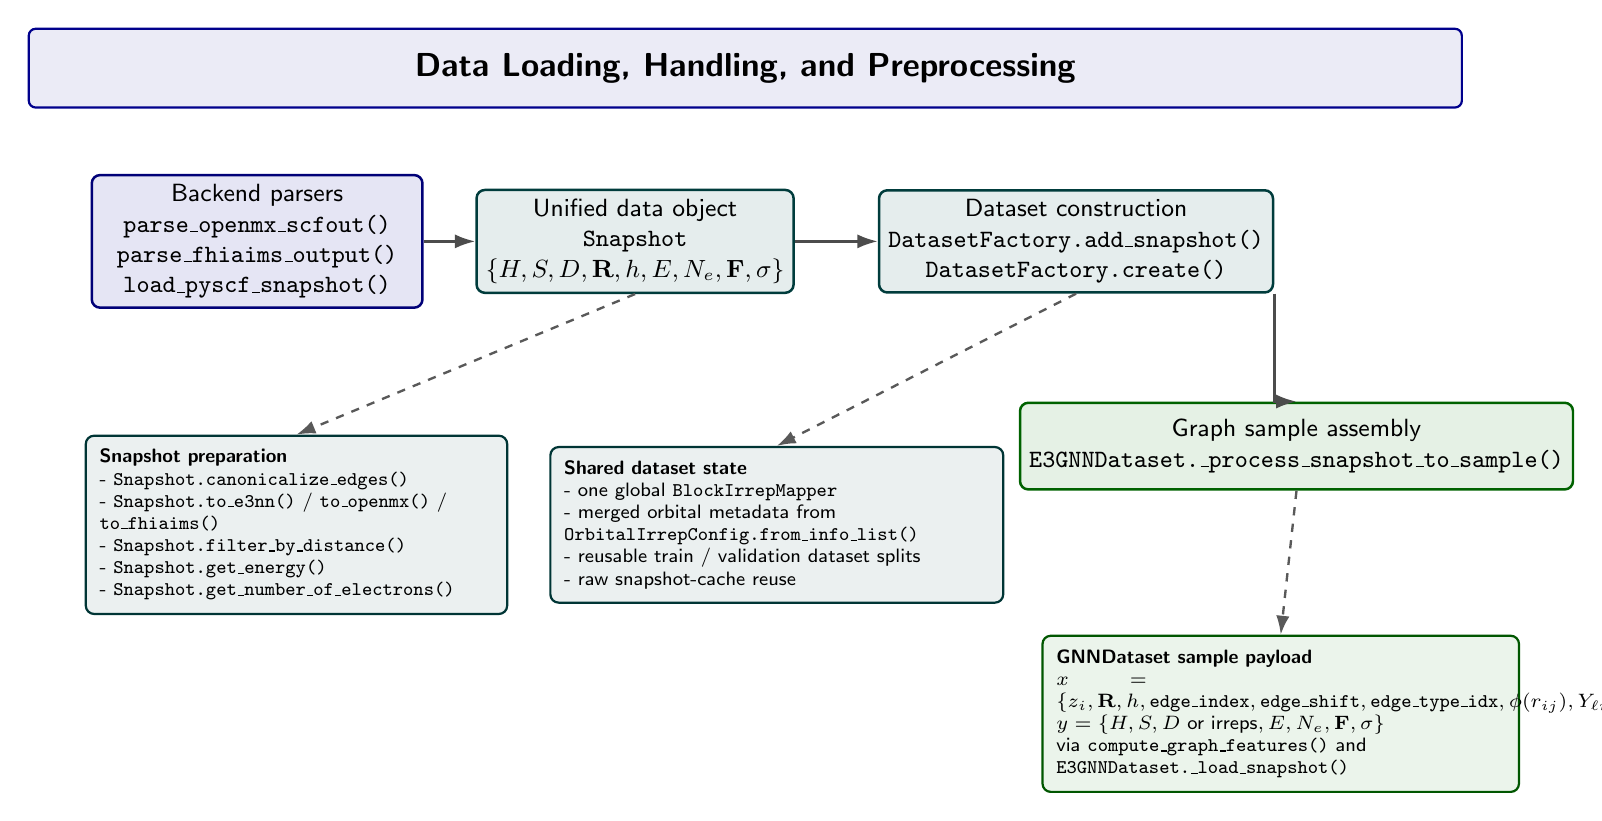
\begin{tikzpicture}[x=1cm,y=1cm]

\node[titlebox, minimum width=18.2cm] (title) at (0,0) {Data Loading, Handling, and Preprocessing};

% Abstract logical structure:
% parsers -> Snapshot objects -> dataset factory / shared mapper -> GNNDataset samples

\node[stage=mandalaBlue, minimum width=4.2cm] (parse) at (-6.2,-2.2)
{Backend parsers\\
\texttt{parse\_openmx\_scfout()}\\
\texttt{parse\_fhiaims\_output()}\\
\texttt{load\_pyscf\_snapshot()}};

\node[stage=mandalaTeal, minimum width=4.0cm] (snap) at (-1.4,-2.2)
{Unified data object\\
\texttt{Snapshot}\\
$\{H,S,D,\mathbf R,h,E,N_e,\mathbf F,\sigma\}$};

\node[stage=mandalaTeal, minimum width=4.3cm] (factory) at (4.2,-2.2)
{Dataset construction\\
\texttt{DatasetFactory.add\_snapshot()}\\
\texttt{DatasetFactory.create()}};

\node[stage=mandalaGreen, minimum width=4.8cm] (dataset) at (7.0,-4.8)
{Graph sample assembly\\
\texttt{E3GNNDataset.\_process\_snapshot\_to\_sample()}};

\draw[arrow] (parse) -- (snap);
\draw[arrow] (snap) -- (factory);
\draw[arrow] (factory.south east) |- (dataset.north);

\node[sidepanel=mandalaTeal, text width=5.0cm] (snap_panel) at (-5.7,-5.8)
{\textbf{Snapshot preparation}\\
- \texttt{Snapshot.canonicalize\_edges()}\\
- \texttt{Snapshot.to\_e3nn()} / \texttt{to\_openmx()} / \texttt{to\_fhiaims()}\\
- \texttt{Snapshot.filter\_by\_distance()}\\
- \texttt{Snapshot.get\_energy()}\\
- \texttt{Snapshot.get\_number\_of\_electrons()}};

\node[sidepanel=mandalaTeal, text width=5.4cm] (factory_panel) at (0.4,-5.8)
{\textbf{Shared dataset state}\\
- one global \texttt{BlockIrrepMapper}\\
- merged orbital metadata from \texttt{OrbitalIrrepConfig.from\_info\_list()}\\
- reusable train / validation dataset splits\\
- raw snapshot-cache reuse};

\node[sidepanel=mandalaGreen, text width=5.7cm] (dataset_panel) at (6.8,-8.2)
{\textbf{GNNDataset sample payload}\\
$x=\{z_i,\mathbf R,h,\texttt{edge\_index},\texttt{edge\_shift},\texttt{edge\_type\_idx},\phi(r_{ij}),Y_{\ell m}(\hat{\mathbf r}_{ij})\}$\\
$y=\{H,S,D \text{ or irreps},E,N_e,\mathbf F,\sigma\}$\\
via \texttt{compute\_graph\_features()} and \texttt{E3GNNDataset.\_load\_snapshot()}};

\draw[dashedarrow] (snap.south) -- (snap_panel.north);
\draw[dashedarrow] (factory.south) -- (factory_panel.north);
\draw[dashedarrow] (dataset.south) -- (dataset_panel.north);

\end{tikzpicture}
\end{document}
